\subsection{Electromagnetic Induction} 

%\DTMnewdatestyle{dateupdated}{〈definition 〉

Answers to M\Alph{subsection} problems are on page \pageref{induction_prob_answers}.  \textbf{\textcolor{red}{Updated \DTMnow.}}


%--------------------------------------------------------------------------------------------------------------
\figuretoright{0.35}{M_problems/induction/flux_through_rectangle.pdf}{%
\begin{Exercise}
\label{flux_through_rectangle_problem}
An infinitely long (or at least really, really long) straight wire carries current $I_1$. 
A nearby rectangular loop of wire has dimensions $w \times h$ and is a distance $d$ from the first wire.  
(a)~Find the magnetic flux $\Phi_B$ through the rectangular loop due to the current $I_1$.  
(b)~Suppose that the current $I_1$ is increasing linearly with time according to $I_1(t)=\alpha t+ I_0$, where $\alpha$ is a positive constant.  What is the magnitude of the emf in the rectangular loop? 
Hint on part~(a): what would be the bit o' flux $d\Phi_B$ through the thin rectangular sliver with bit o' width $dr$ highlighted on the figure in green?
\end{Exercise}
\begin{Answer}
(a) $\displaystyle \Phi_B = \frac{\mu_0 I_1 h}{2\pi} \ln \left( \frac{d+w}{d}\right)$
(b) $\displaystyle {\cal E} = \frac{\mu_0 \alpha h}{2\pi} \ln \left( \frac{d+w}{d}\right)$
\end{Answer}
}

%--------------------------------------------------------------------------------------------------------------
\begin{Exercise}
The figure below shows a top view of a metal bar that is sliding on two frictionless rails in an external magnetic field applied into the page.
  
\begin{minipage}[t]{0.60\textwidth} 
\begin{enumerate}[labparts]
\item What is the magnetic flux $\Phi_B$ through the shaded loop at the instant shown? 
\item If the bar is moving to the right at speed $v$, what is the magnitude of the induced emf  ${\cal E}$ in the rectangular loop?  Hint: What is the relationship between $x$ and $v$? 
\item What is the magnitude of the induced current $I$ through the loop?  
\item Does the induced current flow clockwise or counterclockwise?  
\end{enumerate}
\end{minipage}
\begin{minipage}[t]{0.39\textwidth} 
\vspace{-0.10in}
\hspace{\fill}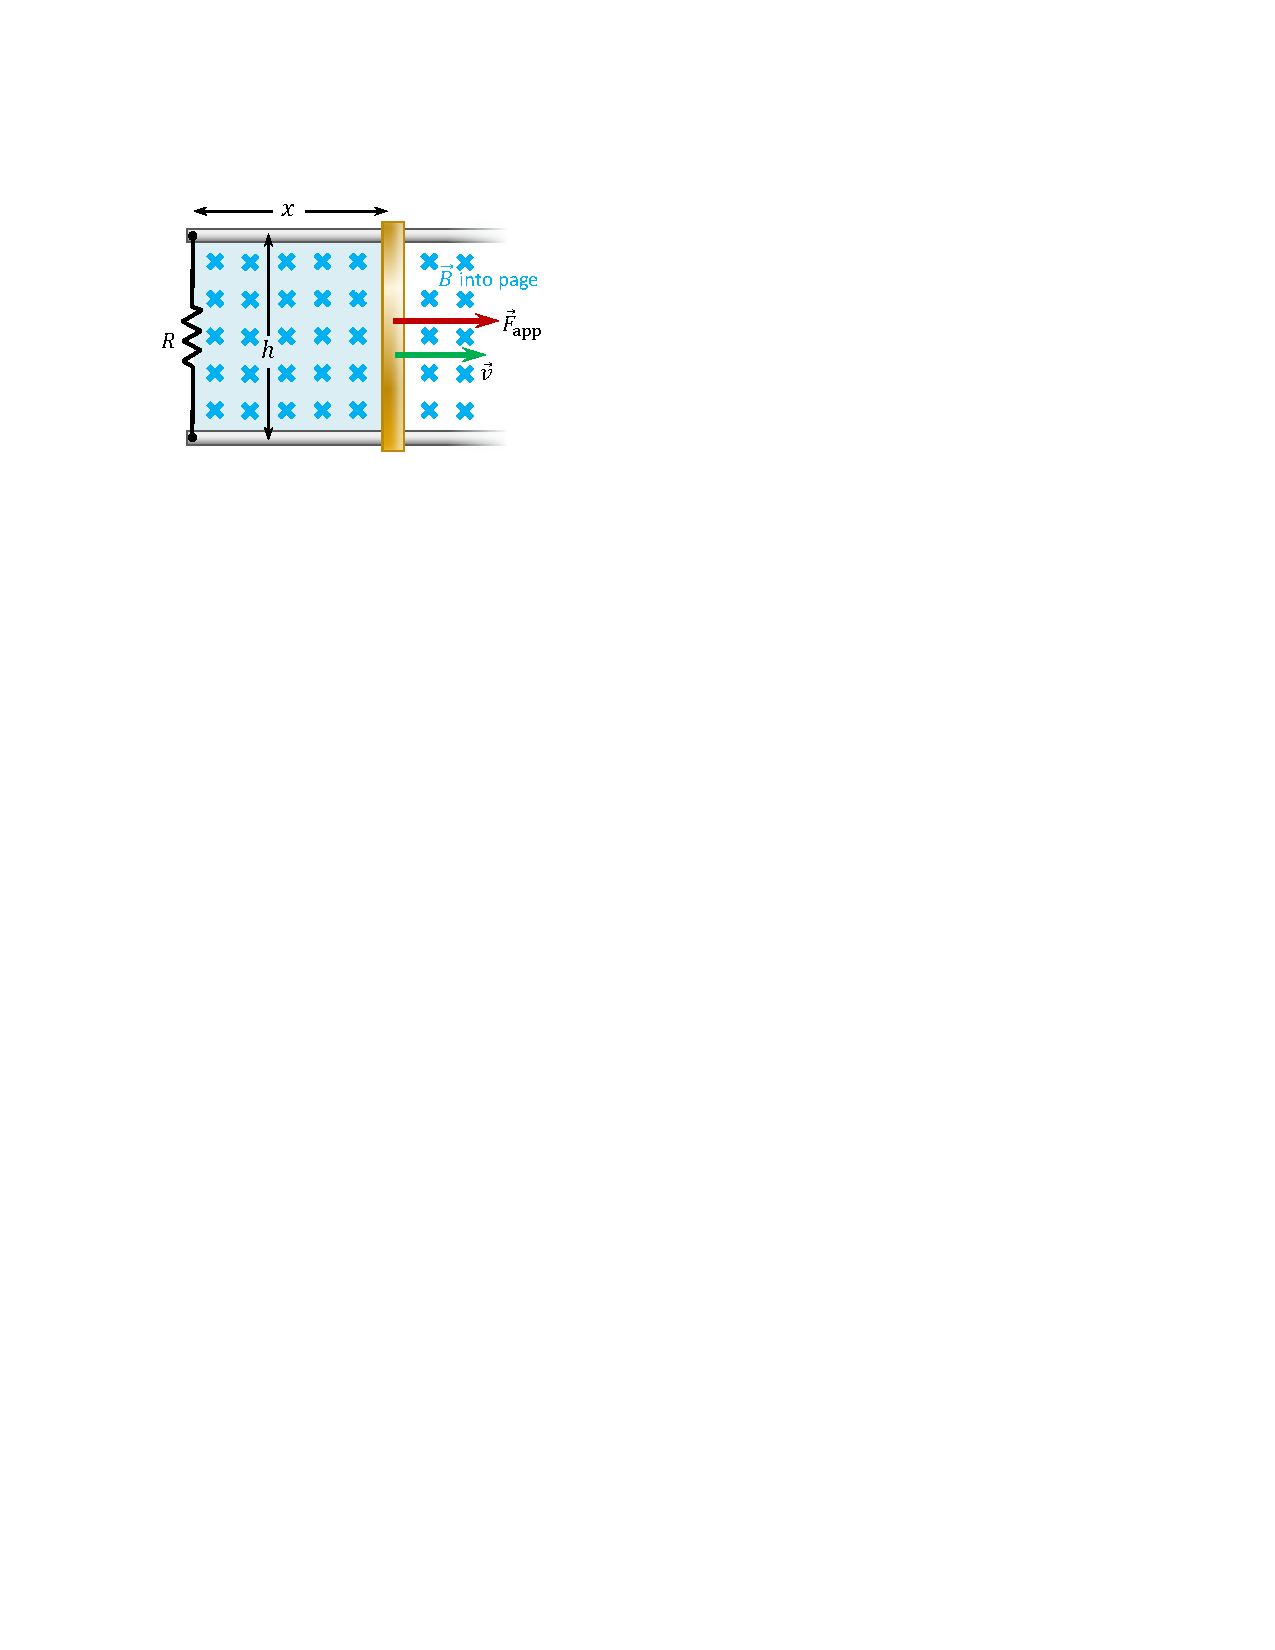
\includegraphics[scale=0.93]{M_problems/induction/bar_on_rails.pdf}
\vspace{-0.20in}
\end{minipage}
\begin{enumerate}[labparts, start=5]
\item Given that you just found the current $I$ through the bar, find the magnitude and direction of the force of the external magnetic field on that current-carrying bar. 
\item What magnitude of applied force $F_\text{app}$ (say, by your hand) is required to keep the bar moving at a constant velocity $\vec{v}\,$?
\item Find the work $W_\text{hand}$ done by your hand in moving the bar a distance $\Delta x$.  
\item The time for the bar to move a distance $\Delta x$ is $\Delta t=\Delta x/v$.  Starting with the expression for power $P=IV$, find the total energy dissipated in the resistor $R$ as heat, $\Delta E_\text{thermal}$.  
\item How do your answers for parts g and h compare? 
\end{enumerate}  
\end{Exercise}
\begin{Answer}
(a)~$\Phi_B =  B h x$
(b)~${\cal E} = B h v$
(c)~$I = B h v / R$
(d)~counterclockwise
(e)~$F=B^2 h^2 v / R$, to the left
(f)~$F_\text{app}=B^2 h^2v / R$
(g)~$W_\text{hand}=B^2 h^2v \Delta x / R$
(i)~$W_\text{hand}$ and $\Delta E_\text{thermal}$ really \textit{should} be the same, or else you've violated conservation of energy.
\end{Answer}


%--------------------------------------------------------------------------------------------------------------
\figuretoright{0.30}{M_problems/induction/solenoid_and_circle_coil.pdf}{%
\begin{Exercise}
A circular coil of 15 turns of wire and a radius of $R=10$~cm is placed around a long solenoid of radius 2~cm and 1000 turns per meter.  The current in the solenoid is $I(t)=I_0 \sin(\omega t)$, where $I_0=5$~amps and $\omega=120$~rad/sec.  Find the emf ${\cal E}(t)$ induced in the circular coil as a function of time.
\end{Exercise}
\begin{Answer}
${\cal E}=(-14.2~\text{mV})\cos(\omega t)$
\end{Answer}

%--------------------------------------------------------------------------------------------------------------
\begin{Exercise}
What is the direction of the induced current in problem~\ref{flux_through_rectangle_problem}?
\end{Exercise}
\begin{Answer}
Counterclockwise
\end{Answer}
} %end of figuretoright from previous problem


%--------------------------------------------------------------------------------------------------------------
\begin{Exercise}
A solenoid of radius $R$ and $n$ turns per length carries a current $I(t)=I_\text{max} \sin(\omega t)$.  (The figure below shows a cutaway view of the solenoid; the real thing would be a full cylinder.)  Find the amplitude of the electric field $E(t)$ at points A and B on the figure.  
\begin{center}
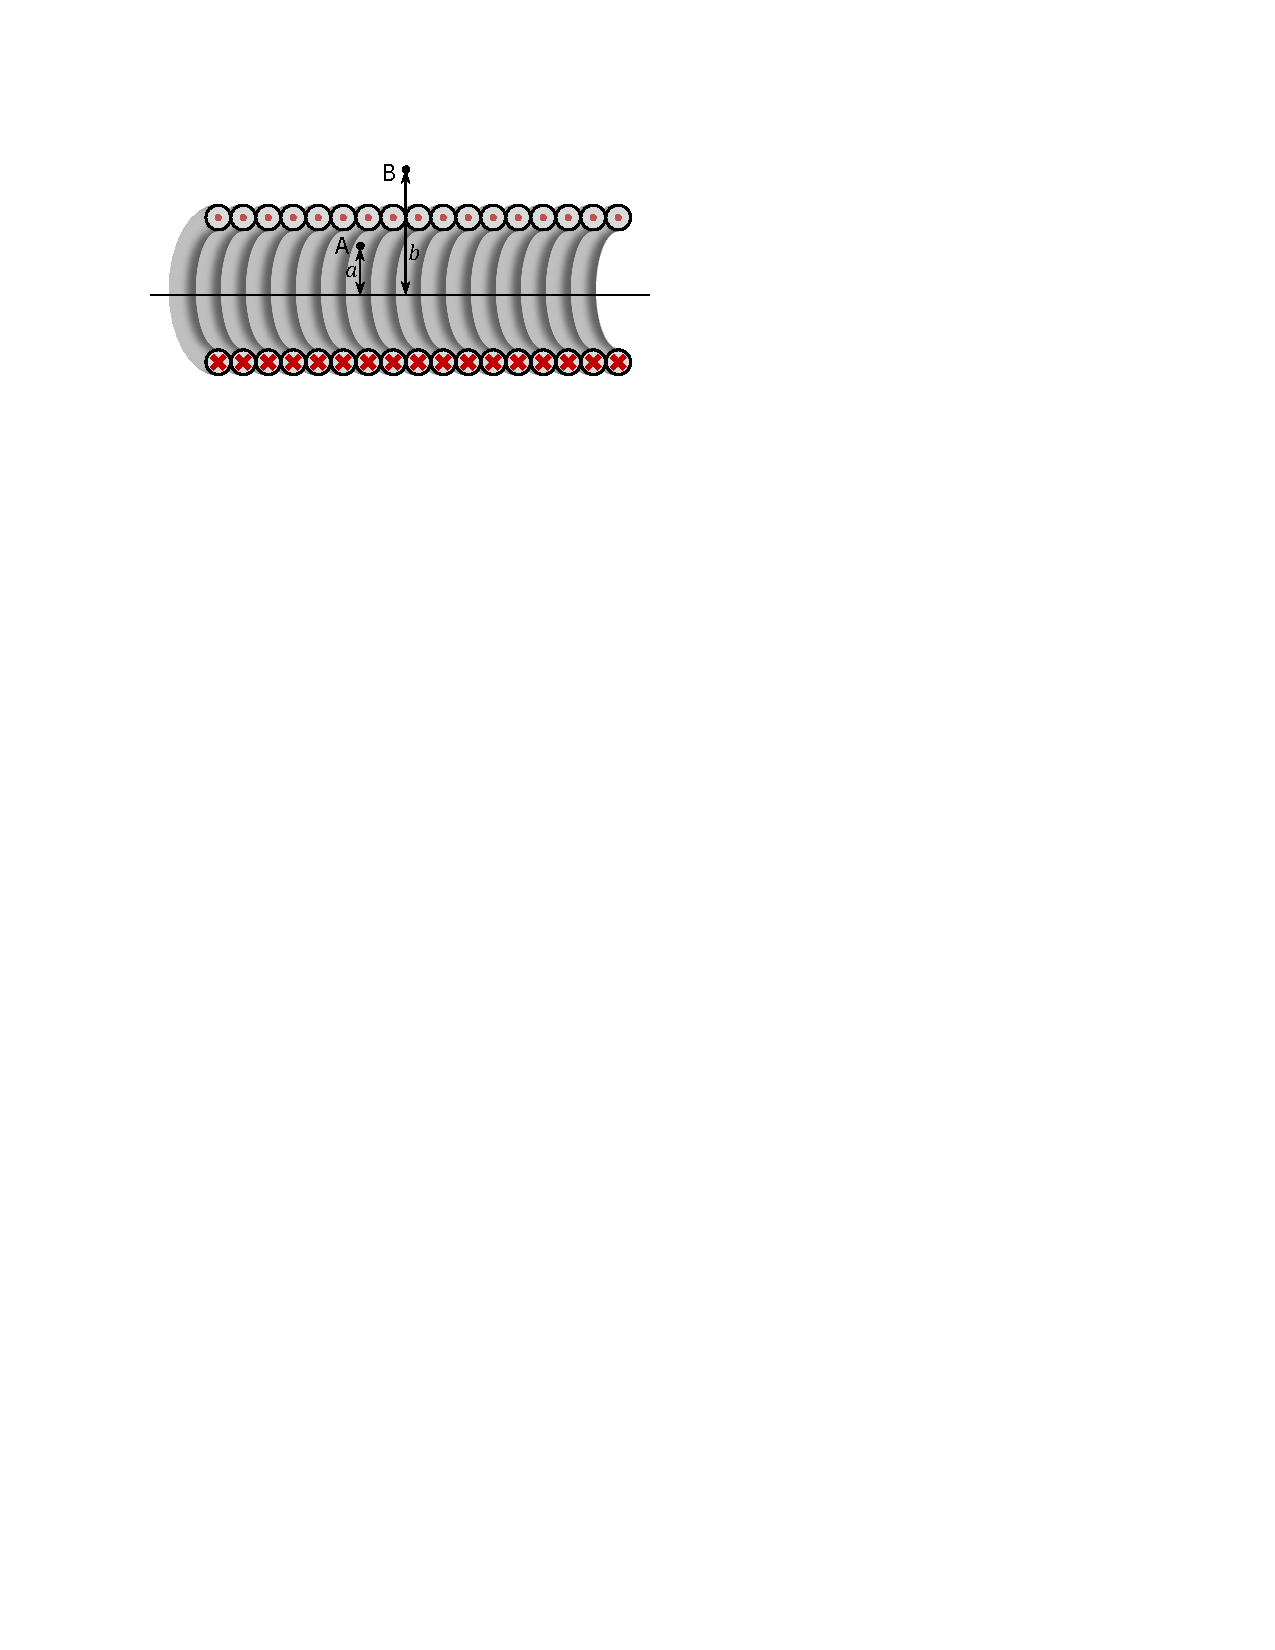
\includegraphics{M_problems/induction/solenoid_cutaway.pdf}
\end{center}

\end{Exercise}
\begin{Answer}
Point A: $E(t) = \frac{1}{2} \mu_0 an\omega I_\text{max}\cos(\omega t)$; 
Point B: $E(t) = \frac{1}{2b} \mu_0 R^2n\omega I_\text{max}\cos(\omega t)$
\end{Answer}


\figuretoright{0.3}{M_problems/induction/falling_magnet.pdf}{
%--------------------------------------------------------------------------------------------------------------
\begin{Exercise}
A bar magnet with its north pole down falls towards a circular metal ring.  
(a)~Draw the field lines you would expect for the bar magnet.  
(b)~As the magnet approaches the ring, does the induced current in the ring flow clockwise or counterclockwise (as seen from above)?  
(c)~Does the induced current attract or repel the bar magnet?  
(d)~After the magnet has fallen through the ring and is falling away from it, does the induced current in the ring flow clockwise or counterclockwise?  
(e)~Does the induced current in the previous part attract or repel the bar magnet?
\end{Exercise}
\begin{Answer}
(b) counterclockwise (c) repel (d) clockwise (e) attract
\end{Answer}

%--------------------------------------------------------------------------------------------------------------
\begin{Exercise}
The figure below on the left shows a circular area in which a uniform magnetic field $\vec{B}$ is directed into the page, increasing according to $B(t)=\alpha t+B_0$, where $\alpha$ is a positive constant.  
(a)~Find the magnitude and direction of the induced electric field $\vec{E}$ at points $P_1$ and $P_2$.
\end{Exercise}
\begin{Answer}
At $P_1: \vec{E} = \frac{1}{2} \alpha r_1$ to the left; 
At $P_2: \vec{E}= \frac{1}{2} \alpha R^2/r_2$ up, towards the top of the page.
\end{Answer}
} %end of figuretoright from previous problem


\hspace{\fill}
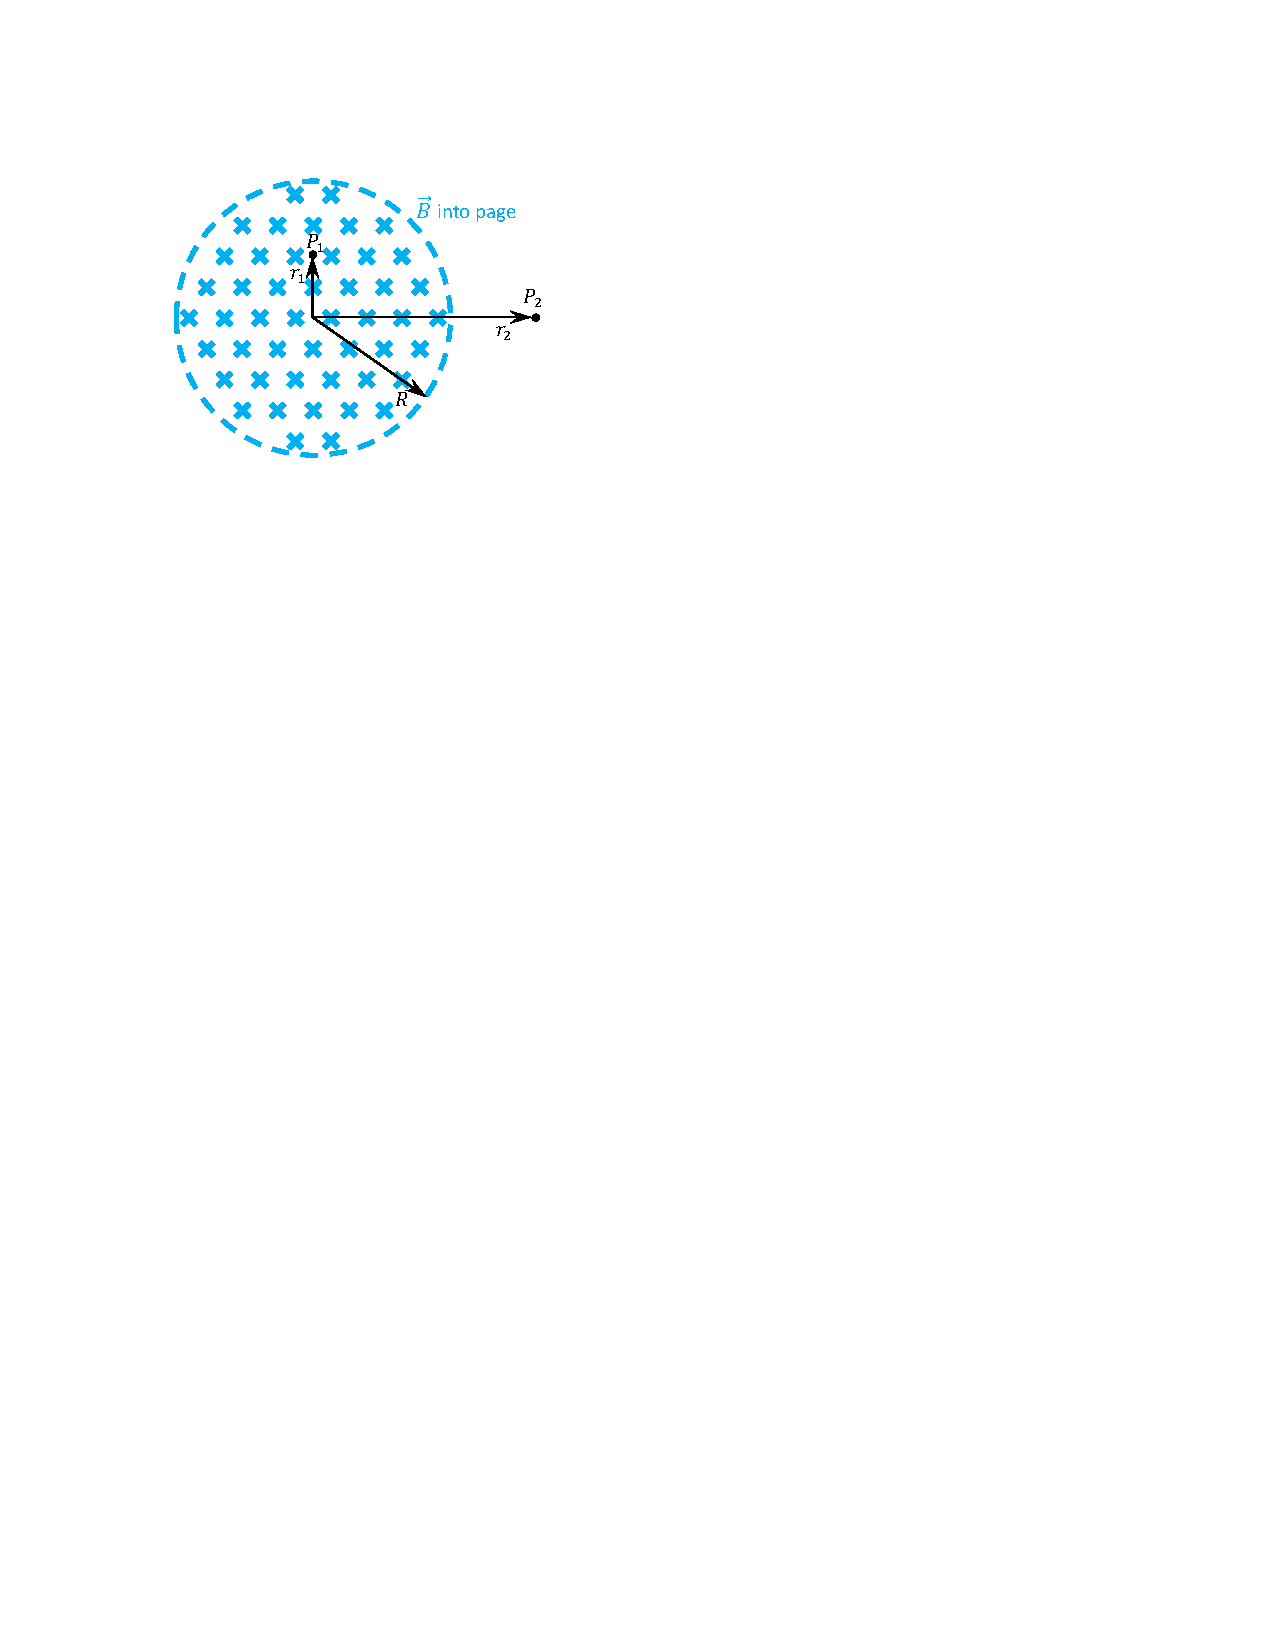
\includegraphics{M_problems/induction/circle_of_B_field.pdf}
\hspace{\fill}
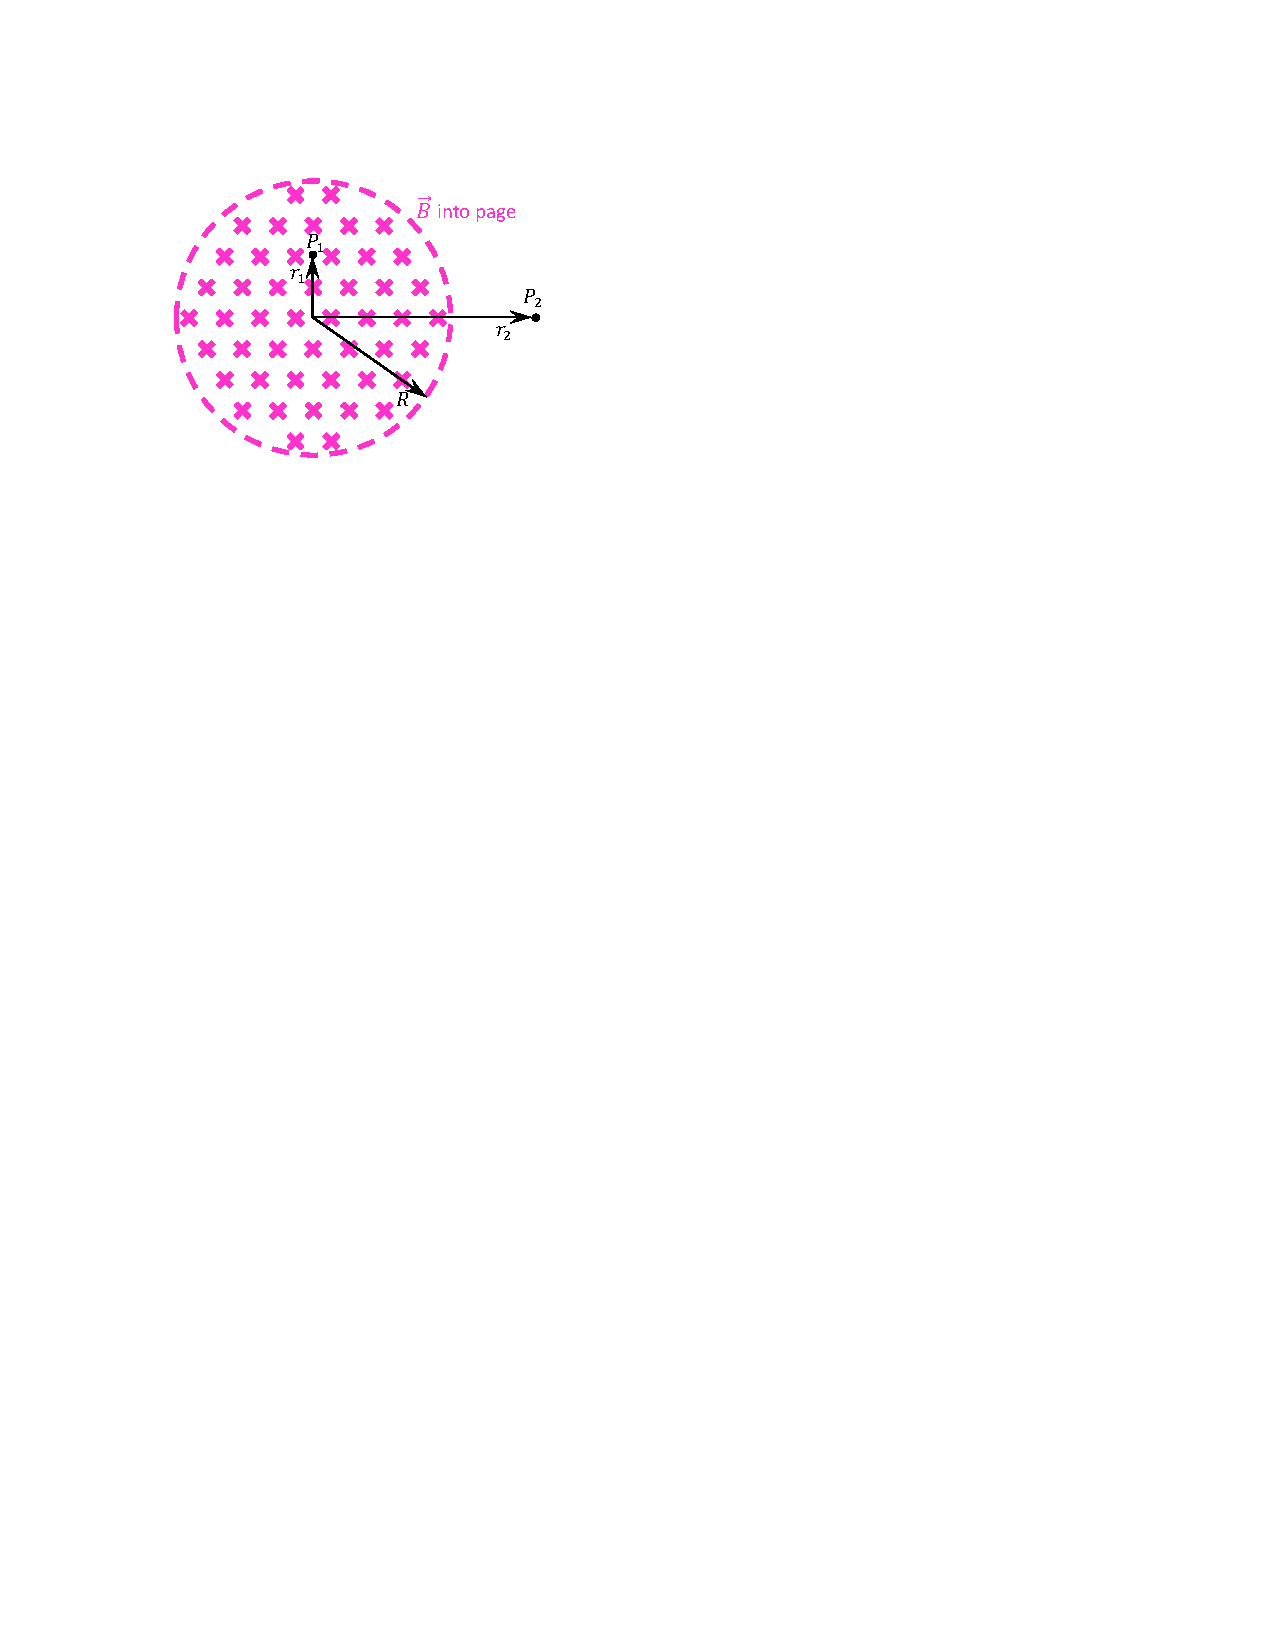
\includegraphics{M_problems/induction/circle_of_E_field.pdf}
\hspace{\fill}


%--------------------------------------------------------------------------------------------------------------
\begin{Exercise}
The figure above on the right shows a circular area in which a uniform magnetic field $\vec{E}$ is directed into the page, increasing according to $E(t)=\alpha t+E_0$, where $\alpha$ is a positive constant.  
(a)~Find the magnitude and direction of the induced magnetic field $\vec{B}$ at points $P_1$ and $P_2$.
\end{Exercise}
\begin{Answer}
At $P_1: \vec{B} = \frac{1}{2} \mu_0 \epsilon_0 \alpha r_1$ to the right; 
At $P_2: \vec{B} = \frac{1}{2}\alpha \mu_0 \epsilon_0 R^2/r_2$ down, towards the bottom of the page.
\end{Answer}


%--------------------------------------------------------------------------------------------------------------
\begin{Exercise}
A ``Rogowski coil'' is a long, flexible solenoid that can be bent into a circle around a wire carrying an AC current $I(t)$, as shown in the figure, to measure the amplitude of the current.  
Suppose the coil has n turns per unit length, and the cross-sectional area of the solenoid (actually more like a toroid) is A.
\figuretoright{0.30}{M_problems/induction/rogowski_coil.pdf}{%
\begin{enumerate}[labparts]
\item If the current in the wire to be measured is $I(t)=I_\text{max}  \sin(\omega t)$, what is the amplitude 
${\cal E}_\text{max}$ of the emf induced in the Rogowski coil?  
\item The Rogowski coil is easy to use, because 
(1)~the wire being measured doesn't have to be in the center of the coil, and 
(2)~the coil does not respond to current in other nearby wires that it does not enclose.  Why are these two things true?
\end{enumerate} 
}
Hints on part (a): How many turns are there in a short length of the coil $ds$? If the magnetic flux through a single coil is $BA$, what would be the net flux through a short length of the coil $ds$?
\end{Exercise}
\begin{Answer}
(a) $E_\text{max}=\mu_0 nA\omega I_\text{max}$ (b) In part (a), you used Amp\`ere's law to equate the line integral of $B$ to the enclosed current.  Amp\`ere's law is true for any path, and the line integral only depends on the current enclosed.
\end{Answer}


\vspace{0.7in}

\textbf{Answers to Selected {\thesubsection} Problems:}
\label{induction_prob_answers}
%\shipoutExercise
\shipoutAnswer

\cleardoublepage
